
% $Header: /cvsroot/latex-beamer/latex-beamer/solutions/generic-talks/generic-ornate-15min-45min.en.tex,v 1.5 2007/01/28 20:48:23 tantau Exp $

\documentclass[smaller, hyperref={colorlinks=true}]{beamer}
\mode<presentation>
{
  \usetheme{Singapore}
  \usefonttheme[onlymath]{serif}
  % or ...
 %  \setbeamercovered{transparent}
  % or whatever (possibly just delete it)
}


\usepackage[czech]{babel}
% or whatever

\usepackage[utf8]{inputenc}
\usepackage{fancyvrb}
\usepackage{multicol}

% or whatever

%\usepackage{times}
%\usepackage[T1]{fontenc}
% Or whatever. Note that the encoding and the font should match. If T1
% does not look nice, try deleting the line with the fontenc.


\title{PAS 01 - Exploratory statistics}

\author{Jan B\v rezina}
\institute % (optional, but mostly needed)
{
  %\inst{2}%
  Technical University of Liberec
}


% If you wish to uncover everything in a step-wise fashion, uncomment
% the following command: 

%\beamerdefaultoverlayspecification{<+->}

% ***************************************** SYMBOLS
\def\div{{\rm div}}
\def\Lapl{\Delta}
\def\grad{\nabla}
\def\supp{{\rm supp}}
\def\dist{{\rm dist}}
%\def\chset{\mathbbm{1}}
\def\chset{1}

\def\Tr{{\rm Tr}}
\def\sgn{{\rm sgn}}
\def\to{\rightarrow}
\def\weakto{\rightharpoonup}
\def\imbed{\hookrightarrow}
\def\cimbed{\subset\subset}
\def\range{{\mathcal R}}
\def\leprox{\lesssim}
\def\argdot{{\hspace{0.18em}\cdot\hspace{0.18em}}}
\def\Distr{{\mathcal D}}
\def\calK{{\mathcal K}}
\def\FromTo{|\rightarrow}
\def\convol{\star}
\def\impl{\Rightarrow}
\DeclareMathOperator*{\esslim}{esslim}
\DeclareMathOperator*{\esssup}{ess\,sup}
\DeclareMathOperator{\ess}{ess}
\DeclareMathOperator{\osc}{osc}
\DeclareMathOperator{\curl}{curl}

%\def\Ess{{\rm ess}}
%\def\Exp{{\rm exp}}
%\def\Implies{\Longrightarrow}
%\def\Equiv{\Longleftrightarrow}
% ****************************************** GENERAL MATH NOTATION
\def\Real{{\rm\bf R}}
\def\Rd{{{\rm\bf R}^{\rm 3}}}
\def\RN{{{\rm\bf R}^N}}
\def\D{{\mathbb D}}
\def\Nnum{{\mathbb N}}
\def\Measures{{\mathcal M}}
\def\d{\,{\rm d}}               % differential
\def\sdodt{\genfrac{}{}{}{1}{\rm d}{{\rm d}t}}
\def\dodt{\genfrac{}{}{}{}{\rm d}{{\rm d}t}}

\def\vc#1{\mathbf{\boldsymbol{#1}}}     % vector
\def\tn#1{{\mathbb{#1}}}    % tensor
\def\abs#1{\lvert#1\rvert}
\def\Abs#1{\bigl\lvert#1\bigr\rvert}
\def\bigabs#1{\bigl\lvert#1\bigr\rvert}
\def\Bigabs#1{\Big\lvert#1\Big\rvert}
\def\ABS#1{\left\lvert#1\right\rvert}
\def\norm#1{\bigl\Vert#1\bigr\Vert} %norm
\def\close#1{\overline{#1}}
\def\inter#1{#1^\circ}
\def\ol#1{\overline{#1}}
\def\ul#1{\underline{#1}}
\def\eqdef{\mathrel{\mathop:}=}     % defining equivalence
\def\where{\,|\,}                    % "where" separator in set's defs
\def\timeD#1{\dot{\overline{{#1}}}}

% ******************************************* USEFULL MACROS
\def\RomanEnum{\renewcommand{\labelenumi}{\rm (\roman{enumi})}}   % enumerate by roman numbers
\def\rf#1{(\ref{#1})}                                             % ref. shortcut
\def\prtl{\partial}                                        % partial deriv.
\def\Names#1{{\scshape #1}}
\def\rem#1{{\parskip=0cm\par!! {\sl\small #1} !!}}

\def\Xint#1{\mathchoice
{\XXint\displaystyle\textstyle{#1}}%
{\XXint\textstyle\scriptstyle{#1}}%
{\XXint\scriptstyle\scriptscriptstyle{#1}}%
{\XXint\scriptscriptstyle\scriptscriptstyle{#1}}%
\!\int}
\def\XXint#1#2#3{{\setbox0=\hbox{$#1{#2#3}{\int}$}
\vcenter{\hbox{$#2#3$}}\kern-.5\wd0}}
\def\ddashint{\Xint=}
\def\dashint{\Xint-}

% ******************************************* DOCUMENT NOTATIONS
% document specific
\def\rh{\varrho}
\def\vl{{\vc{u}}}
\def\th{\vartheta}
\def\vx{\vc{x}}
\def\vX{\vc{X}}
\def\vr{\vc{r}}
\def\veta{\vc{\eta}}
\def\dx{\,\d\vx}
\def\dt{\,\d t}
\def\bulk{\zeta}
\def\cS{\close{S}}
\def\eps{\varepsilon}
\def\phi{\varphi}
\def\Bog{{\mathcal B}}
\def\Riesz{{\mathcal R}}
\def\distr{\mathcal D}
\def\Item{$\bullet$}

\def\MEtst{\mathcal T}
%***************************************************************************

% highlight color
\setbeamercolor{my blue}{fg=blue}
\def\blue#1{{\usebeamercolor[fg]{my blue} #1}}

\setbeamercolor{my green}{fg=green}
\def\green#1{{\usebeamercolor[fg]{my green} #1}}

% color for term definition
\setbeamercolor{my orange}{fg=orange}
\def\df#1{{\usebeamercolor[fg]{my orange} #1}}
\def\xskip{{\vspace{2ex}}}

\begin{document}

\begin{frame}
  \titlepage
\end{frame}


\begin{frame}{Literature} 
\begin{itemize}
 \item Jiří Anděl: Statistické metody, Matfyzpress, 2007, Knihovna
 \item Briš, Litschmannová: Statistika I., skripta VŠB Ostrava, WEB
 \item 
 \item G. J. Kerns: Introduction to Probability and Statistics Using R, WEB
 \item http://www.r-tutor.com/
\end{itemize}
more on the web: morf.matfyz.cz/vyuka/pas
\end{frame}

\begin{frame}{Contents of the course}
 \begin{itemize}
  \item exploratory statistics ( basic data processing, graphs )
  \item basics of probability theory 
  \item statistical analysis (inferential statistics)
  \item statistical software R (minimalistic introduction)
 \end{itemize}
\end{frame}

\begin{frame}{Exploratory statistics}
\begin{itemize}
 \item Detection of errors or incompleteness
 \item Familiarize with new data through:
 \item Getting numerical characteristics (frequency, average, variance)
 \item Visualization
 \item Postulation of hypotheses
\end{itemize}
 
\end{frame}


\begin{frame}{Example: quality of canteen}
\begin{enumerate}
\item WHO would you ask? \\
      \pause
      \blue{full population}  \\
      \hspace{3em}  e.g. all people through whole week/year\\
      \blue{selected sample} \\
      \hspace{3em}  Can we get TRUE random sample? \\
      
\vspace{3ex}      
\item WHAT would you ask? (resulting variables)\\
      \pause 
      \vspace{1ex}
      Do you like the meal? (binary variable)\\
      Mark the quality. (discrete variable)\\
      How much did you spend? (qualitative variable)      
\end{enumerate}

\end{frame}


\begin{frame}{Population and samples (ask who) }
\df{Population} - full set of objects of our interest

citizens of ČR, all visitors of the canteen, all applications of a drug

\xskip

``sampled survey'' - select subset (\df{sample}) of the population

\xskip 
                         
\blue{Advantages:} lower cost, population need not to be accessible,\\
\noindent\hspace{5em} destructive survey

\xskip

Selection of sample :
\begin{itemize}
 \item \df{random sampling} (can be dificult)
 \item \df{stratified random sampling} ( evenly in subgroups, \\ heterogeneous populations )
 \item \df{cluster sampling} hierarchy: random towns, random streets, random citizens
 \item ``voluntary sampling '' DANGER
\end{itemize}
  
\end{frame}

\begin{frame}{Type of statistical quantities (ask what) }

\df{Dependent variable} - we can not control its value\\
\df{Independent variable} - we can control/set the value\\
\hspace{3em}experiment should cover all relevant values

\xskip
\blue{Types of variable values:}
\begin{itemize}
\item \df{qualitative variables}\\
       \begin{itemize}
        \item \df{nominal} - no ordering (logical; colour, drug type)
        \item \df{ordinal} - has ordering (marks)
       \end{itemize} 
\item \df{quantitative variables}\\
      \begin{itemize}
       \item \df{discrete}
         \begin{itemize}
         \item \df{finite} ( number of heads from 10 coin throws, dice throw? )
         \item \df{countable} ( number of radioactive decays per second )
         \end{itemize}
       \item \df{continuous} ( hight, weight )
       \end{itemize}
\end{itemize}

\xskip
Qualitative are also called ``dicrete'' ...\\
... but do not SUM (even if labeled by numbers).
\end{frame}


\begin{frame}{Data representation}
  Try to extract main features of the data

  \begin{itemize}
   \item graphical representation (plots)
   \item numerical representation (characteristics)
   \begin{itemize}
       \item measures of the position/center
       \item measures of variability    
   \end{itemize} 
   \item support for making hypothesis about data
  \end{itemize}
\end{frame}


\section{Qualitative variables}

\begin{frame}{Qualitative data - numerical characteristics}
\blue{Nominal variable}:\\
       (sampled) \df{frequency} $n_i$ of value $i$, $\sum n_i = n$ \\
       (sampled) \df{relative frequency} $p_i=n_i/n$, $\sum p_i = 1$ \\
       \df{modus} - value with maximal frequency

\pause
\xskip

\blue{Ordinal variable}:\\
sorted values: $x_1 < x_2 < \dots < x_n$\\
\df{cumulative frequency}: $m_i = \sum_{j=1}^i n_i$\\
\df{relative cumulative frequency}: $F_i = \sum_{j=1}^i p_i = m_i / n$

\xskip
canonical order of nominal data (for plotting) is by descending frequencies
\end{frame}       


\begin{frame}[fragile]{Nominal data - pie chart}
 \df{ pie chart } with absolute frequencies,
 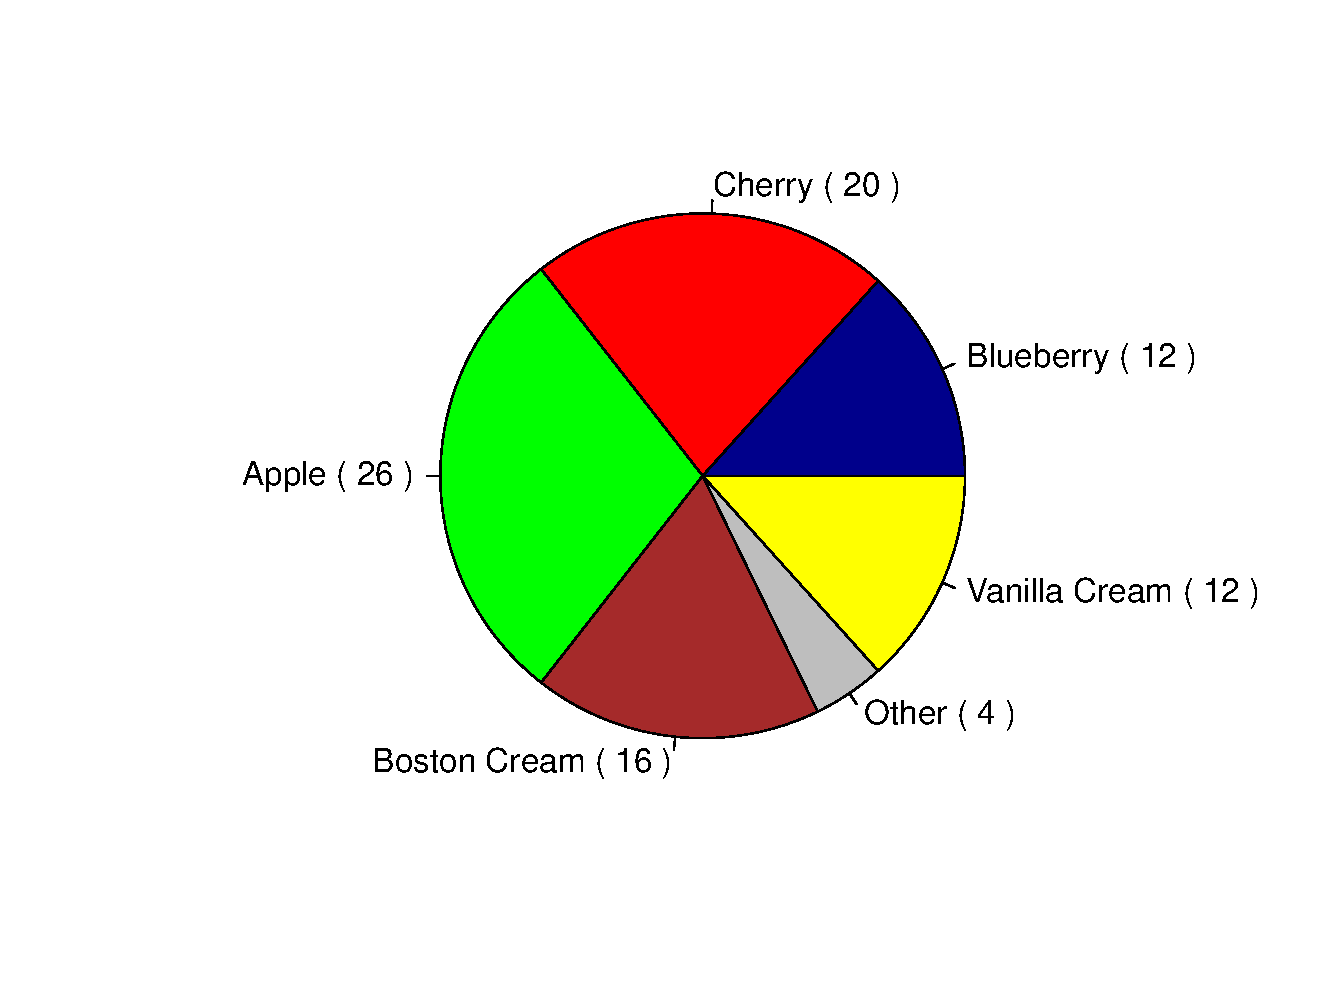
\includegraphics[scale=0.3]{./01_pie_chart.pdf}
 % 01_pie_chart.png: 480x480 pixel, 72dpi, 16.93x16.93 cm, bb=0 0 480 480       

\begin{Verbatim}[fontsize=\scriptsize]
R> pie.sales=c(12,20,26,16,4,12)
R> names(pie.sales) <- c("Blueberry", "Cherry","Apple", "Cream", "Other", "Vanilla")
R> labels=labels=paste(names(pie.sales),"(",pie.sales, ")")
R> pie(pie.sales, labels, col=c("darkblue","red", "green","brown","grey","yellow"))'
\end{Verbatim}
\end{frame}

\begin{frame}[fragile]{Nominal data - bar plot}

\df{ bar plot } absolute frequencies, comparisons of groups

 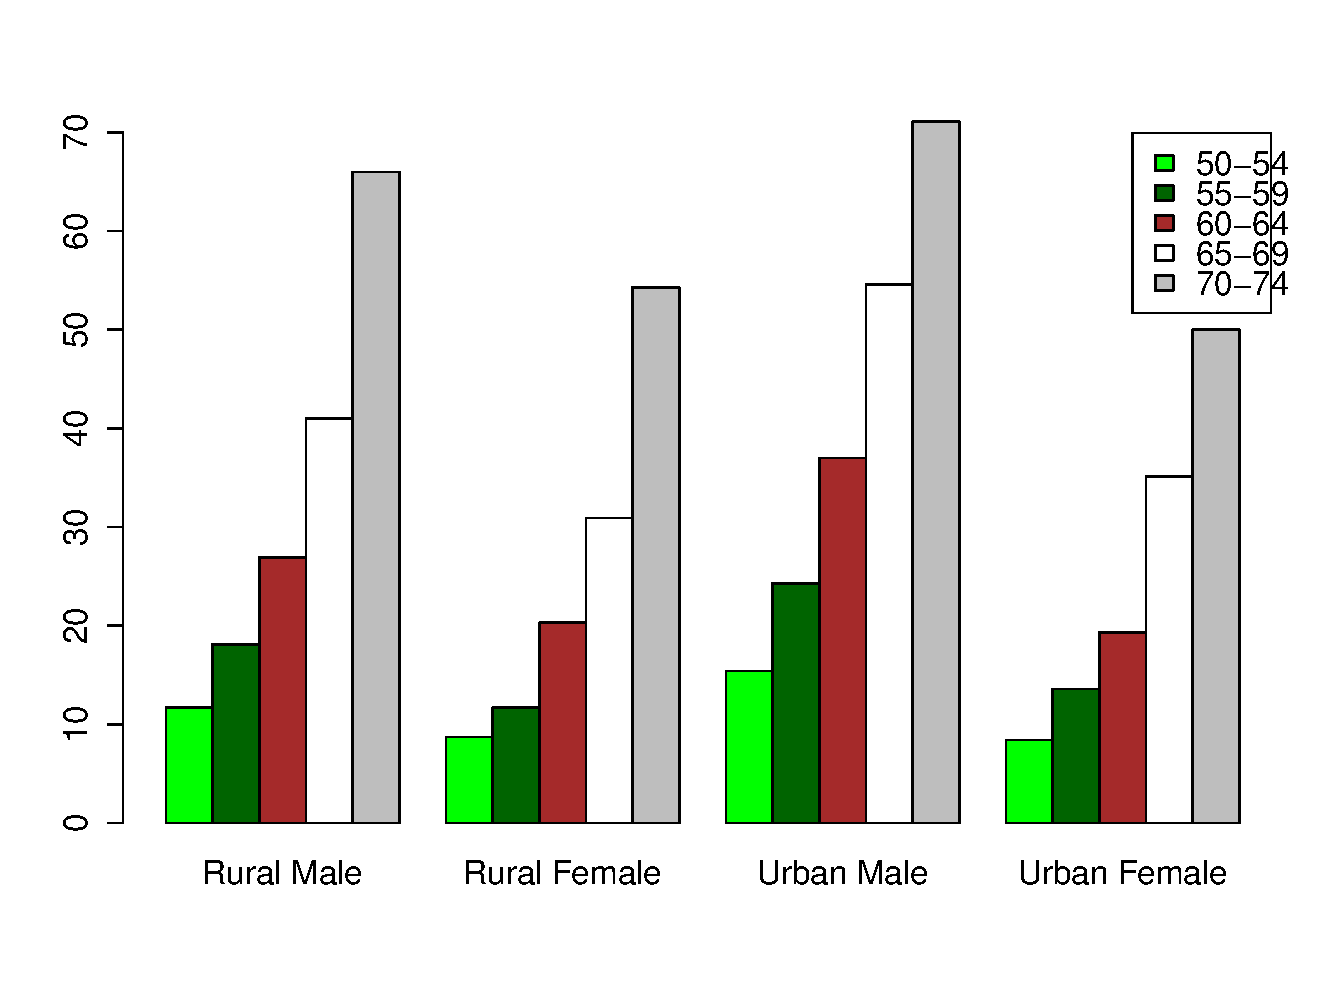
\includegraphics[scale=0.25]{./01_bar_plot.pdf}
% 01_bar_plot.png: 480x480 pixel, 72dpi, 16.93x16.93 cm, bb=0 0 480 480
 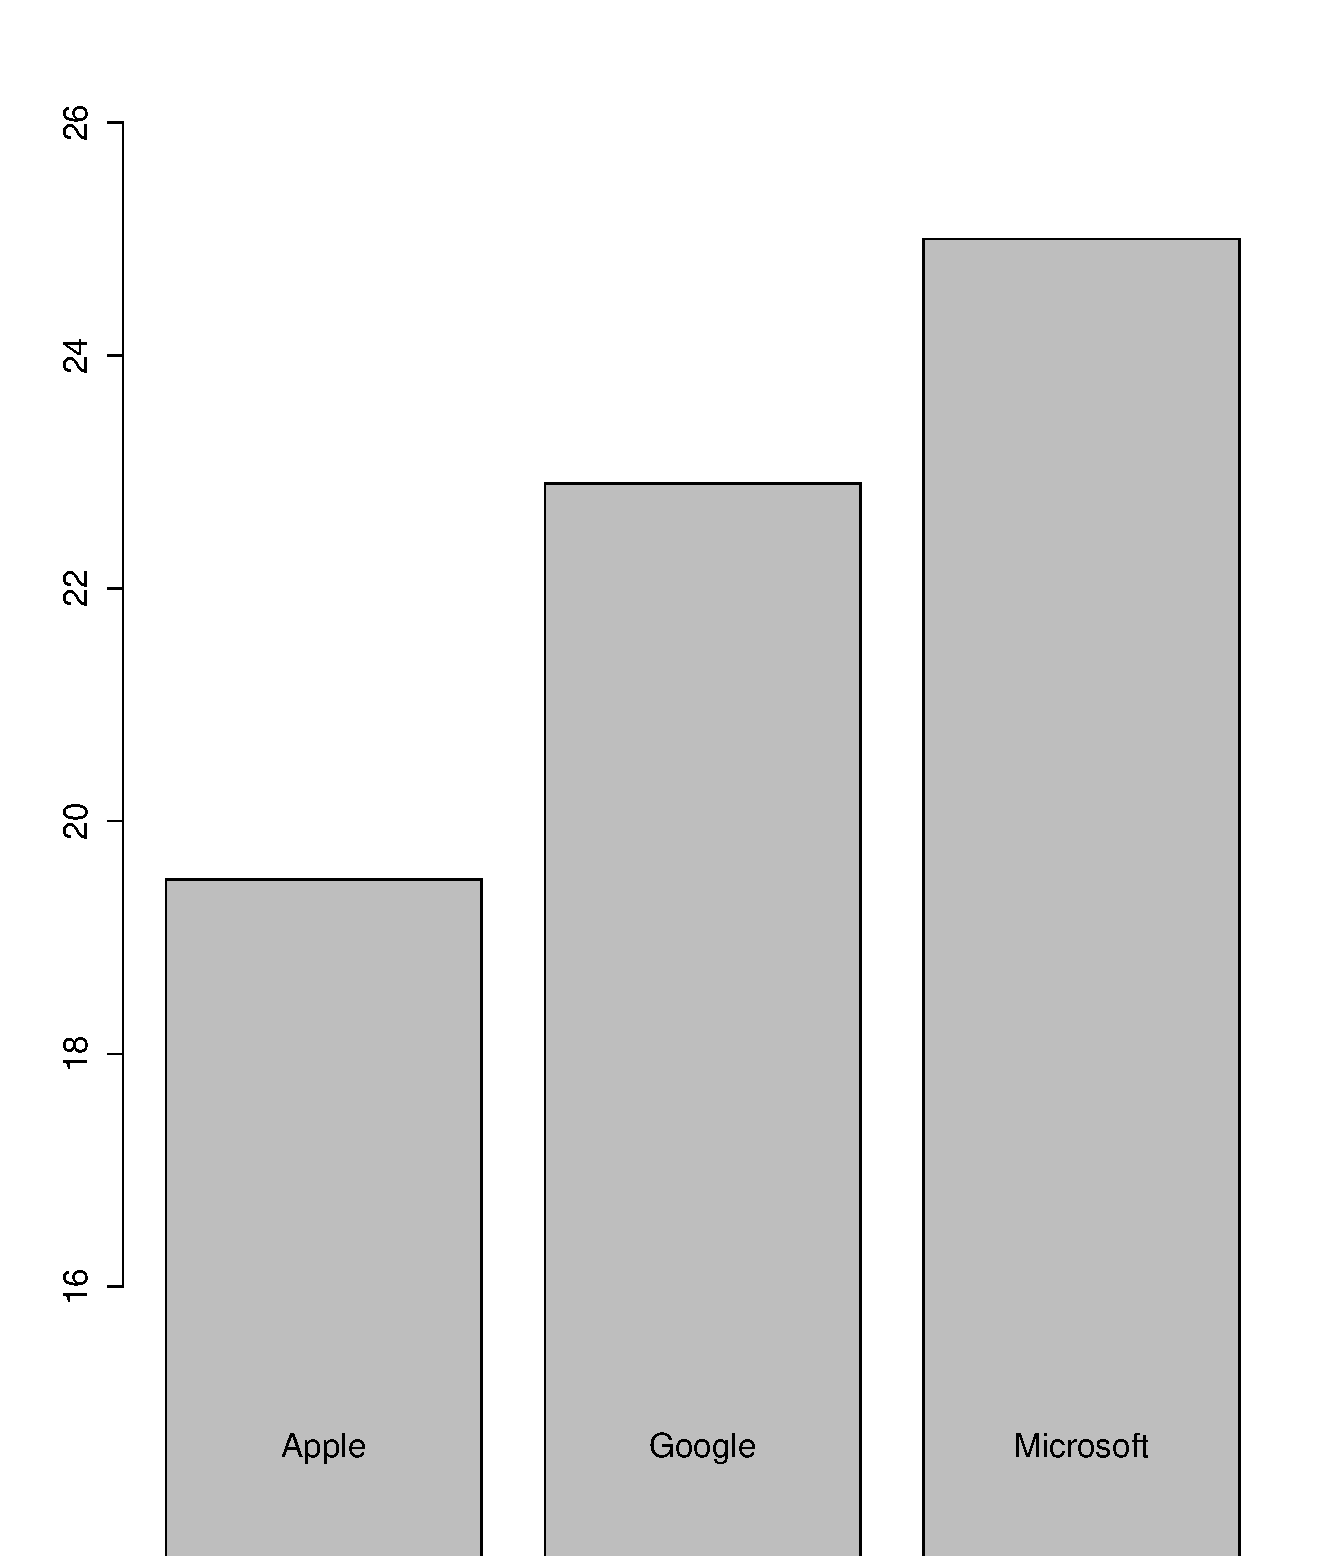
\includegraphics[scale=0.18]{./01_barplot_problem.pdf}
% 01_bar_plot.png: 480x480 pixel, 72dpi, 16.93x16.93 cm, bb=0 0 480 480

\begin{Verbatim}[fontsize=\scriptsize]
R> barplot(VADeaths, beside=T, legend=rownames(VADeaths),
           col=c("green","darkgreen","brown","white","gray") )

R> barplot(c(19.5,22.9,25), names.arg=c("Apple","Google","Microsoft"), ylim=c(15,26))
\end{Verbatim}

 
\end{frame}

\begin{frame}[fragile]{Claveland's plots and lattice graphics}
\noindent
\hbox{
\hspace{-3cm}
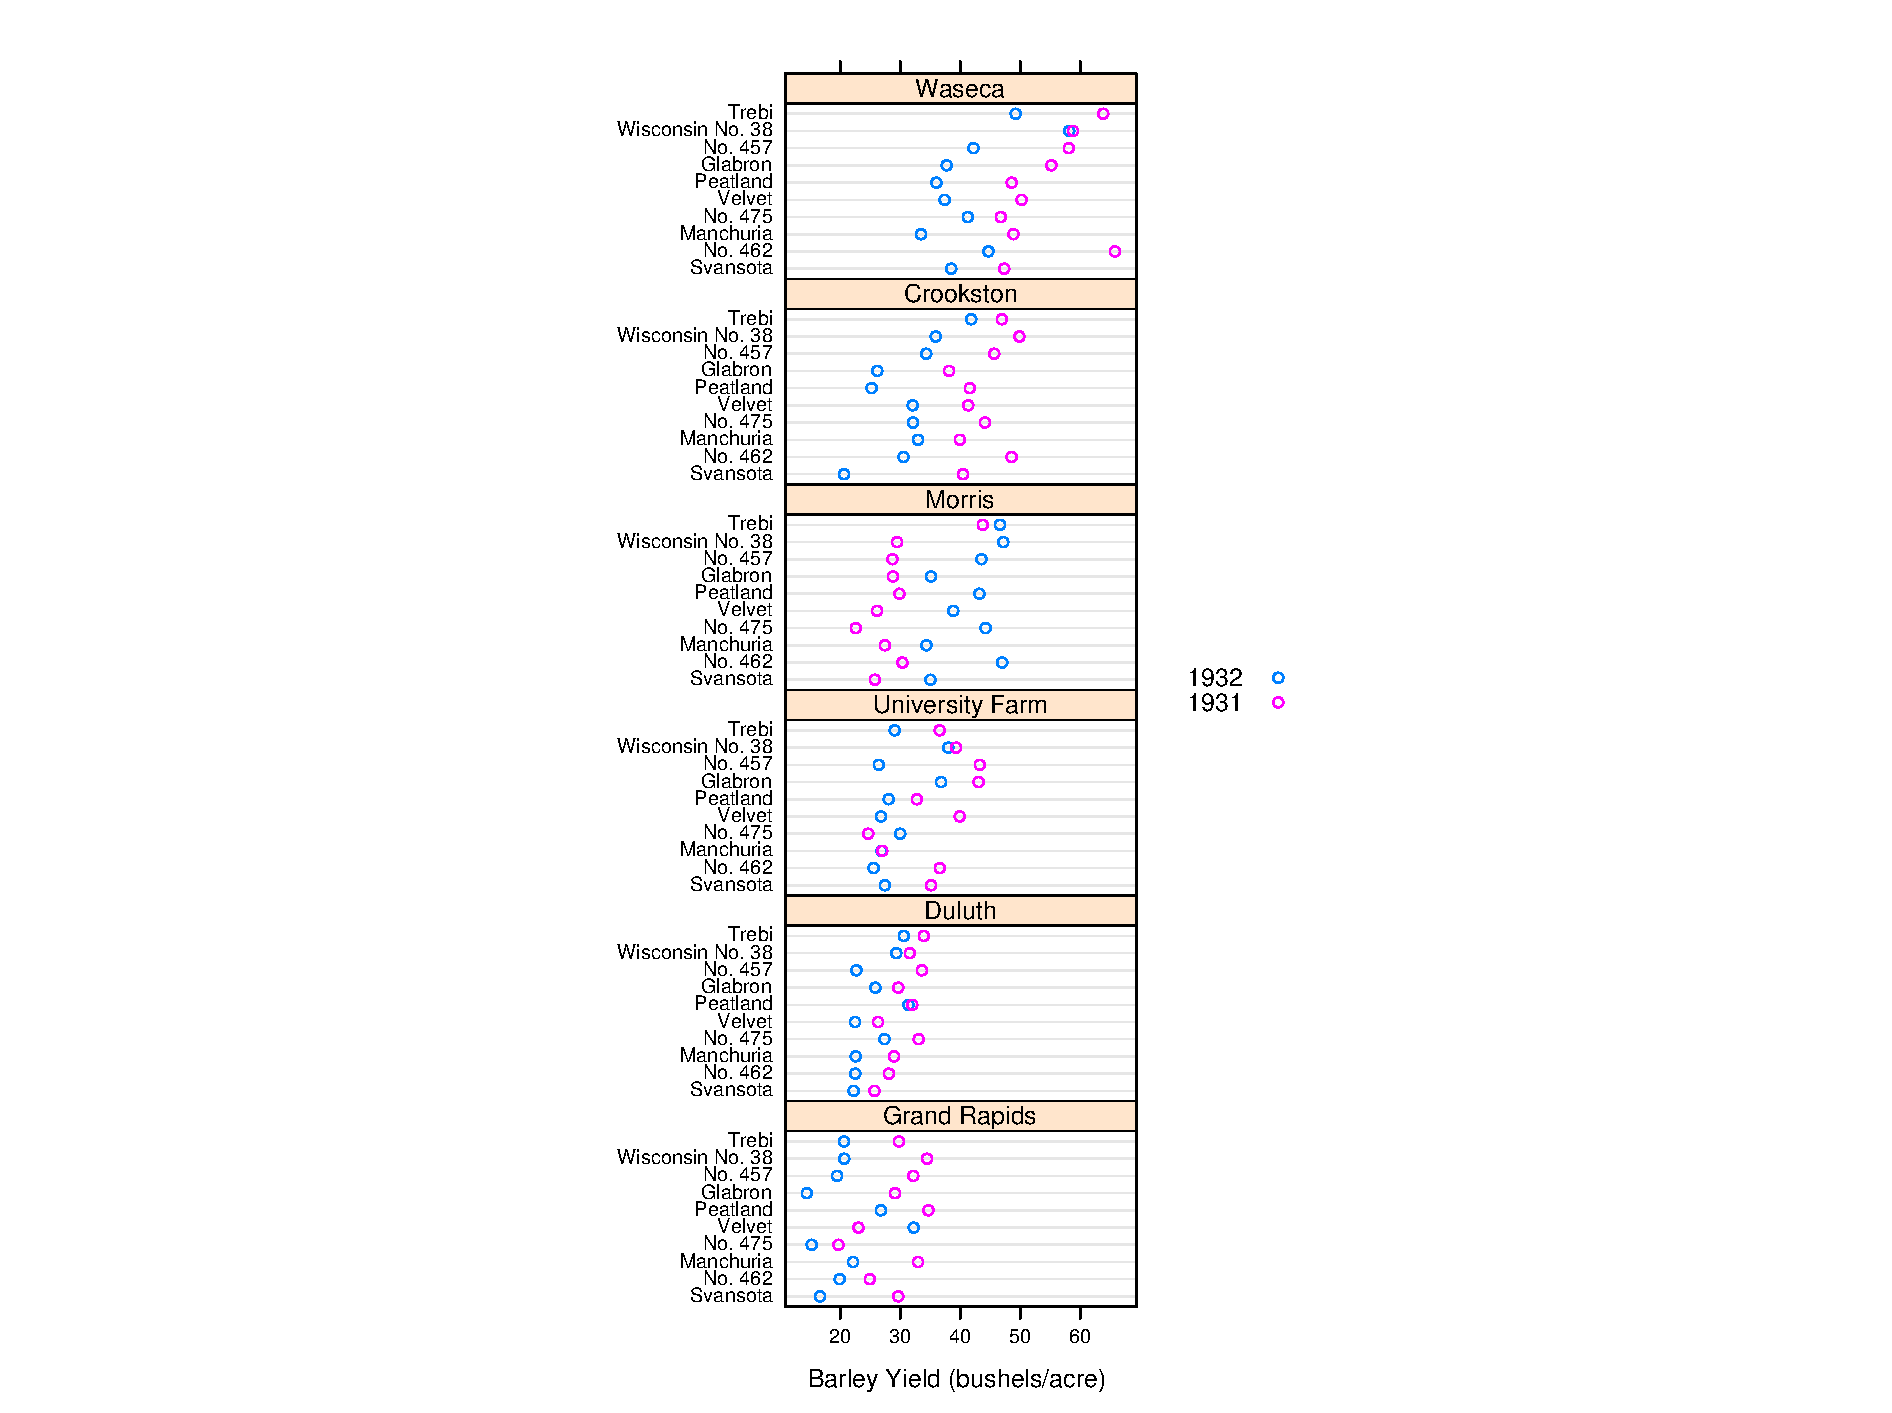
\includegraphics[scale=0.35]{./01_lattice_dotplot.pdf}
\hspace{-3cm}
\vbox{
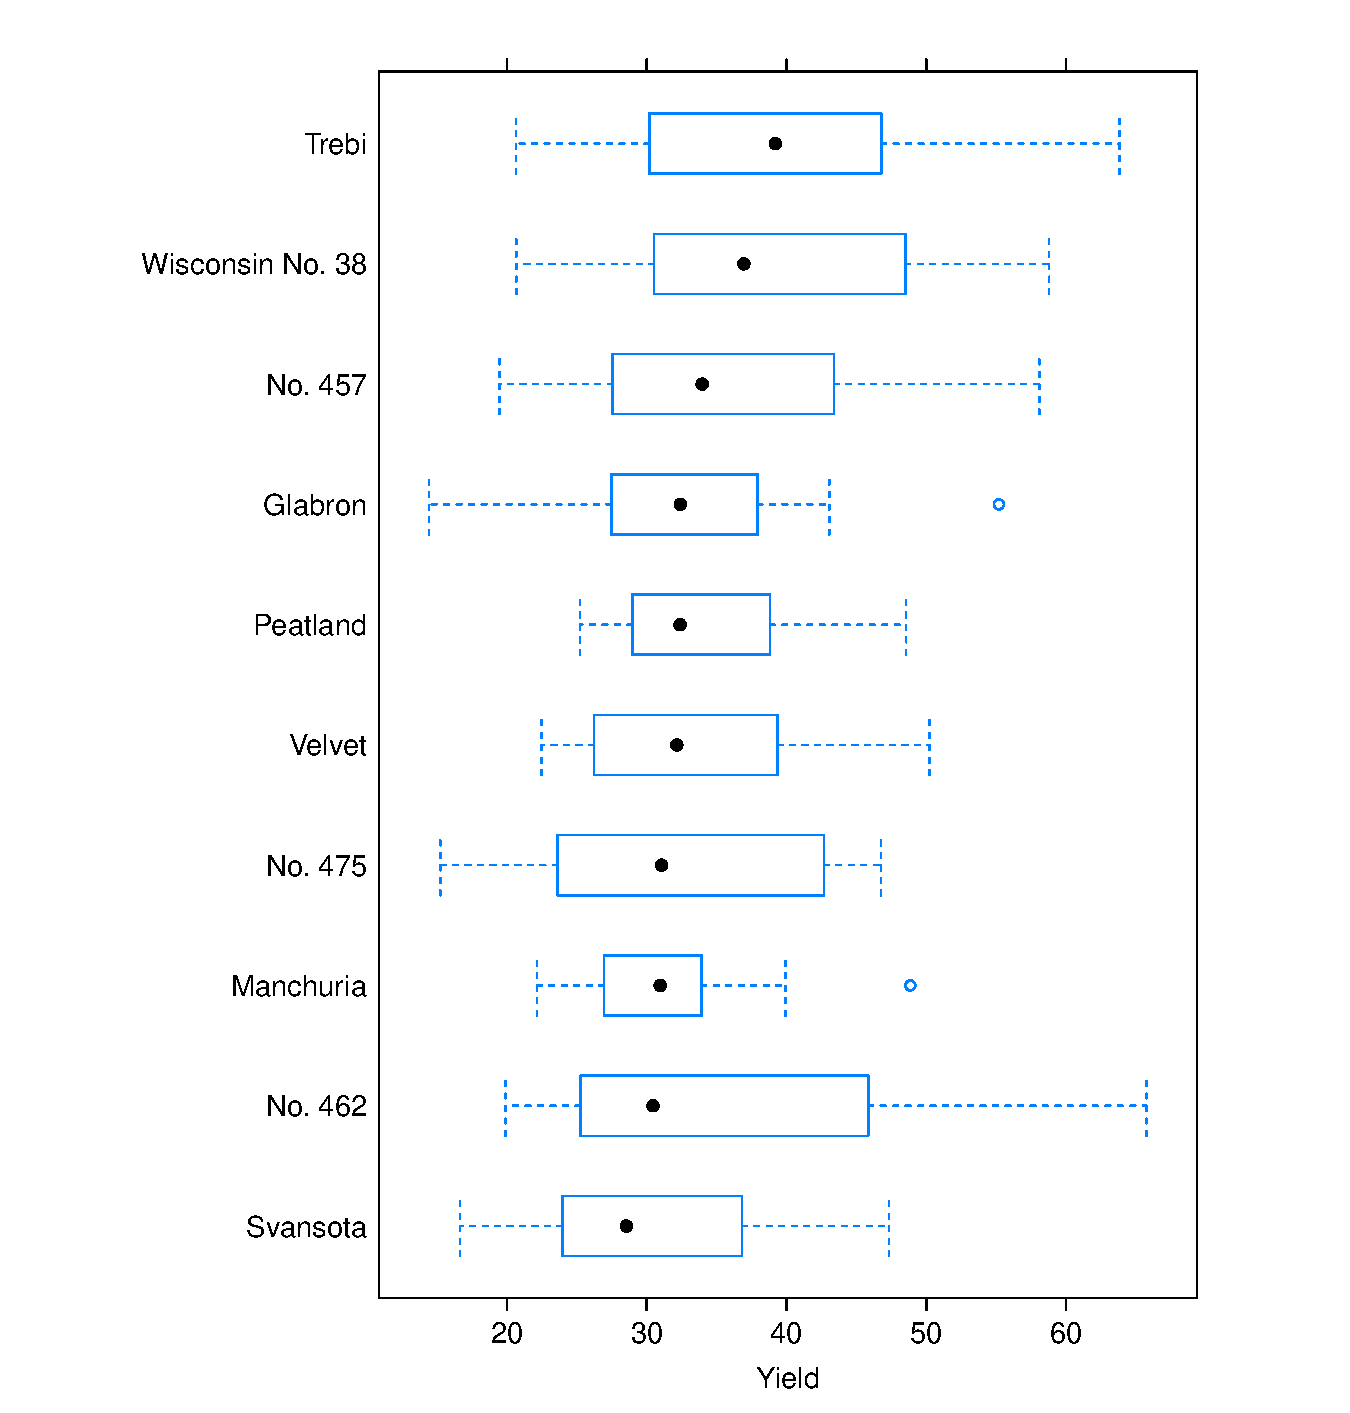
\includegraphics[scale=0.23]{./01_lattice_boxplots.pdf}
\begin{Verbatim}[fontsize=\tiny]
dotplot(variety ~ yield | site, data = barley, groups = year,
        key = simpleKey(levels(barley$year), space = "right"),
        xlab = "Barley Yield (bushels/acre) ",
        aspect=0.5, layout = c(1,6), ylab=NULL)

bwplot(variety~yield,data=barley, aspect=1.5,
       scales=list(
         cex=1.2 ),
       xlab=list(label="Yield",cex=1.2) 
       ) 
\end{Verbatim}

}
}

\end{frame}

   

\begin{frame}{Pareto's plot}
\begin{itemize}
\item barplot of descending absolute frequencies
\item polygon of cumulative frequencies (line plot),\\
\end{itemize}
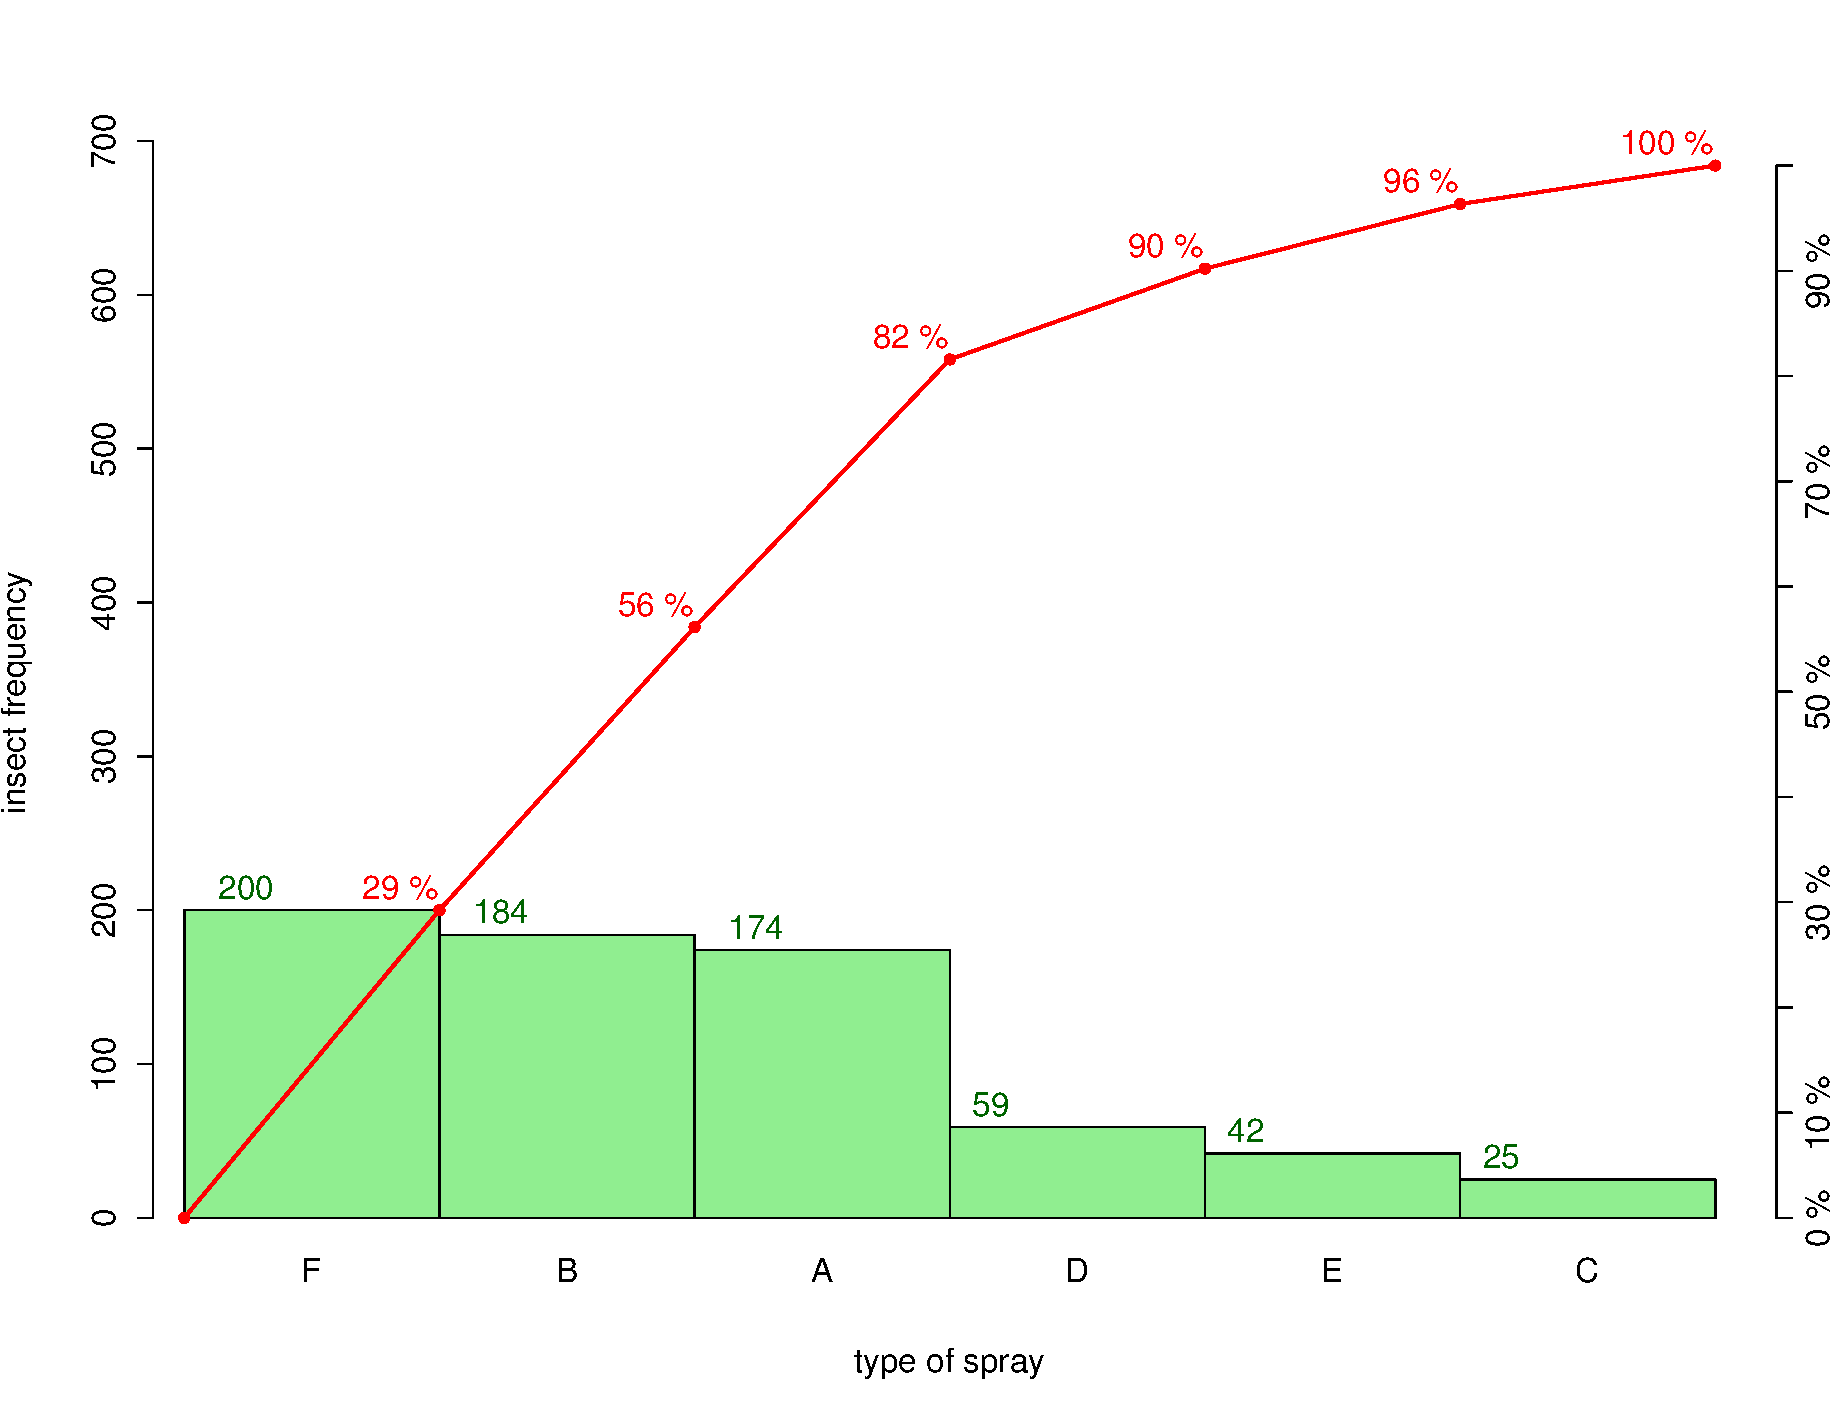
\includegraphics[scale=0.32]{01_pareto.pdf} 
\end{frame}

\begin{frame}[fragile]{...source}
\begin{Verbatim}[fontsize=\scriptsize]
data=colSums(unstack(InsectSprays))

vec=rev(sort(data))
x=0:length(vec)
y=c(0,cumsum(vec))
# empty box + both plots
plot(x,y, type='n',  ylab="insect frequency", xlab="type of spray", axes=FALSE)
barplot(vec,add=T, space=0, col='lightgreen', line=-1)
lines(x,y, type='o', pch=16, col='red', lwd=2)

# cumulative percentage labels in plot
rel_labels=paste(format(100*y/max(y),digits=2, trim=TRUE),"%")
rel_labels[1]=""
text(x,y,rel_labels, adj=c(1,-0.4), col='red')

# cumulative percentage axis on right
ticks=seq(min(y), max(y), length=11)
labels=paste(format(100*ticks/max(ticks),digits=2, trim=TRUE),"%")
axis(4, at=ticks, labels=labels )

# frequency labels on barplot
text(x[-length(x)],vec,format(vec,digits=2, trim=TRUE), adj=c(-0.6,-0.4), col='darkgreen')

########################### automatic alternative
install.packages("qcc")
require(qcc)
pareto.chart(data, las=0)
\end{Verbatim}
\end{frame}





\begin{frame}{Quantitative data}
\blue{measures of center (míry polohy)} : 
\begin{description}
 \item[\df{mean}] $\ol{x} = \frac{1}{n}\sum_i x_i$
 \item[\df{median}] value in the middle in sorted list
 \item[\df{$p$-quantile}] ``value on position $p n$ in sorted list ''
 \item[\df{mode}] (local) maximum of relative frequency/density
 \item[\df{minimum}, \df{maximum}]
\end{description}
%
\blue{measures of spread (míry rozptylu)} : 
\begin{description}
 \item[\df{sample variance}] $\sigma^2 = \frac{1}{n-1} \sum_i (\ol{x} - x_i)^2 = \frac{1}{n-1} \big( \sum_i x_i^2 - n^2\ol{x}^2 \big)$
 \item[\df{sample standard deviation}] $\sigma = \sqrt{\sigma^2}$
 \item[\df{inter quartile range}] $IQR = Q_3 - Q_1 = x_{0.75} - x_{0.25}$
 \item[\df{MAD}] median of absolute deviation from median 
\end{description}
\end{frame}

\begin{frame}[fragile]{Empirical (cumulative) distribution function}

\vspace{-0.7cm}
\hbox{
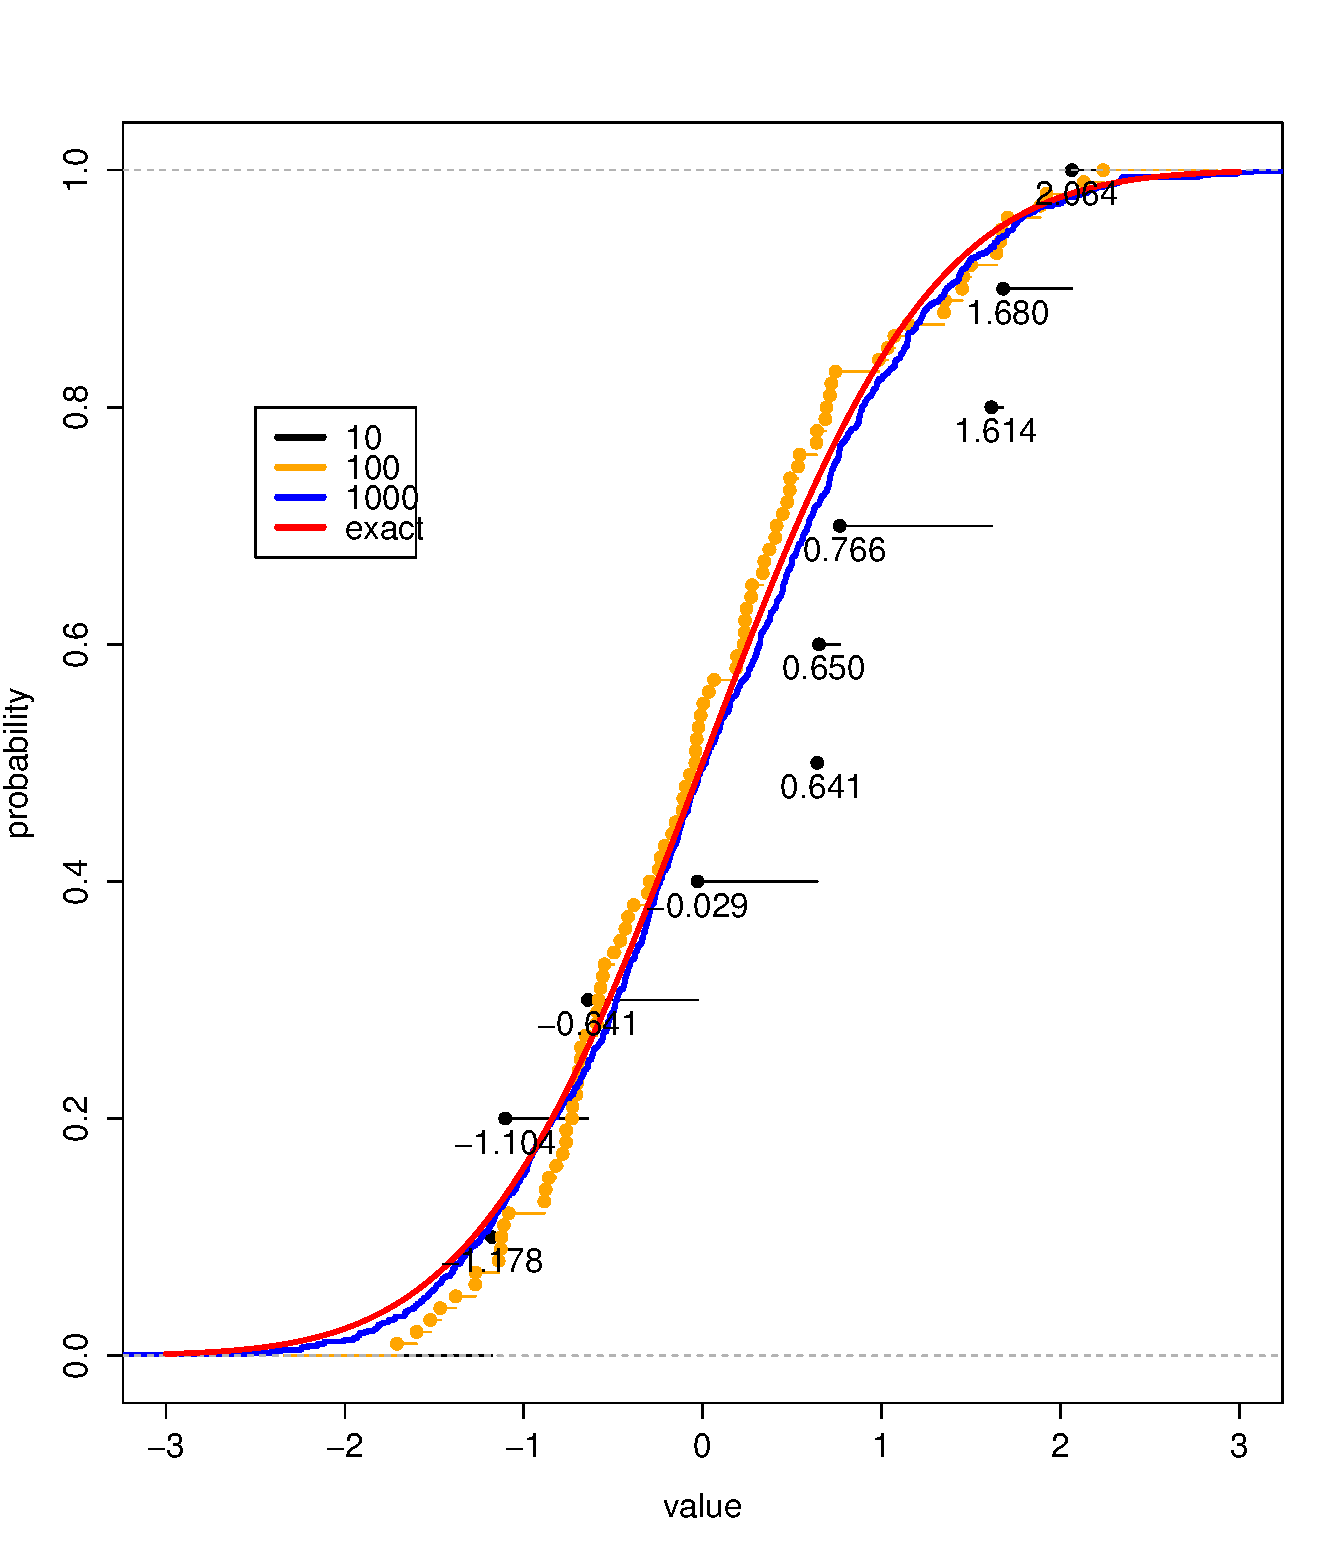
\includegraphics[scale=0.32]{01_ecdf.pdf}
\vbox to \textheight {
\begin{Verbatim}[fontsize=\tiny]
plot(c(-3,3), c(0,1), type="n", 
     xlab="value", ylab="probability")

# ecdf for 10,100, and 1000 samples     
rn10=rnorm(10)
lines(ecdf(rn10) )
lines(ecdf(rnorm(100)), col="orange")
lines(ecdf(rnorm(1000)), col="blue", lwd=3)

# exact distribution function
x=seq(-3,3,0.01)
y=pnorm(x)
lines(x, y, col="red", lwd=3)

# data labels fo 10 samples
text(sort(rn10),1:10/10 - 0.02, 
    format(rn10,digits=2))
    
legend(-2.5,0.8, 
       c("10", "100", "1000", "exact"),
       lty=1, lwd=4,
       col=c("black","orange","blue","red"))
\end{Verbatim}
}
}

\end{frame}


\begin{frame}{Sample Quantiles - possible estimates}
Estimates for $p$-quantile: 
\begin{itemize}
 \item $Q_p = x_{\text{floor}(pn)}$	- inverse of EDF
 \item $Q_p = \frac{x_{\text{ceil}(h)-0.5} + x_{\text{floor}(h)+0.5}}{2}$, $h=pn+0.5$ - same with averaging at jumps
 \item $Q_p = x_{\text{nearest to}(pn)}$ 
 \item $Q_p = x_{\text{floor}(h)} + (h - \text{floor}(h))(x_{1+\text{floor}(h) } - x_{\text{floor}(h)} ) $, $h=(n-1)p+1$ 
\end{itemize} 
\end{frame}


\begin{frame}{Identification of outliers}
value $x$ is outlier if
\begin{enumerate}
\item $x \notin [ Q_1 - 1.5 IQR, Q_3 + 1.5 IQR]$
\item $\abs{z(x)} > 3,\quad z = \frac{x - \overline{X}}{s_X}$, 3 sigma rule
\item MAD coordinate: $\abs{m(x)} > 3, \quad m = \frac{x - x_{0.5}}{1.483 MAD}$
\end{enumerate}

Removing outliers form data ??
\end{frame}

\begin{frame}{Sample skewness and kurtosis}
\df{skewness}:
\[
\alpha = \frac{n}{(n-1)(n-2)}\frac{\sum_{i=1}^{n} (x_i - \overline{x})^3}{s^3}
\]
\df{kurtosis}
\[
\beta = \frac{n(n+1)}{(n-1)(n-2)(n-3)}\frac{\sum_{i=1}{n} (x_i-\overline{x})^4}{s^4} - \frac{3(n-1)^2}{(n-2)(n-3)}
\]
\end{frame}


\section{Graphical representations}

\begin{frame}{Good graphs makes you understand.}
 See the TED talk:\\
 \href{http://www.ted.com/talks/hans_rosling_shows_the_best_stats_you_ve_ever_seen?language=en}{Hans Rosling: The best stats you've ever seen}
\end{frame}


\begin{frame}{Box plot}
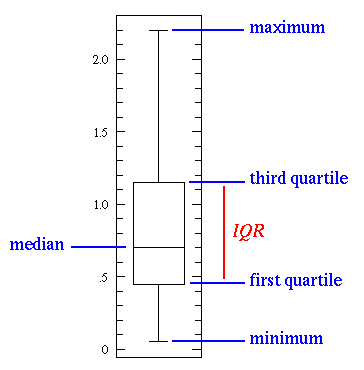
\includegraphics[scale=0.5]{01_simple_box_defs.png} 
\end{frame}


\begin{frame}[fragile]{Histogram}
 \begin{enumerate}
  \item select bins $[x_i, x_{i+1}]$
  \item relative frequencies in bins $q_i$
  \item bar $i$ width $w_i = x_{i+1} - x_i$
  \item bar $i$ height $h_i = q_i / w_i$
 \end{enumerate}
 
 \xskip

 Note: Surface of histogram is always
 \[
   S = \sum_i h_i w_i = \sum_i q_i = 1
 \]

\end{frame}

\begin{frame}
\noindent
\hspace{-3ex}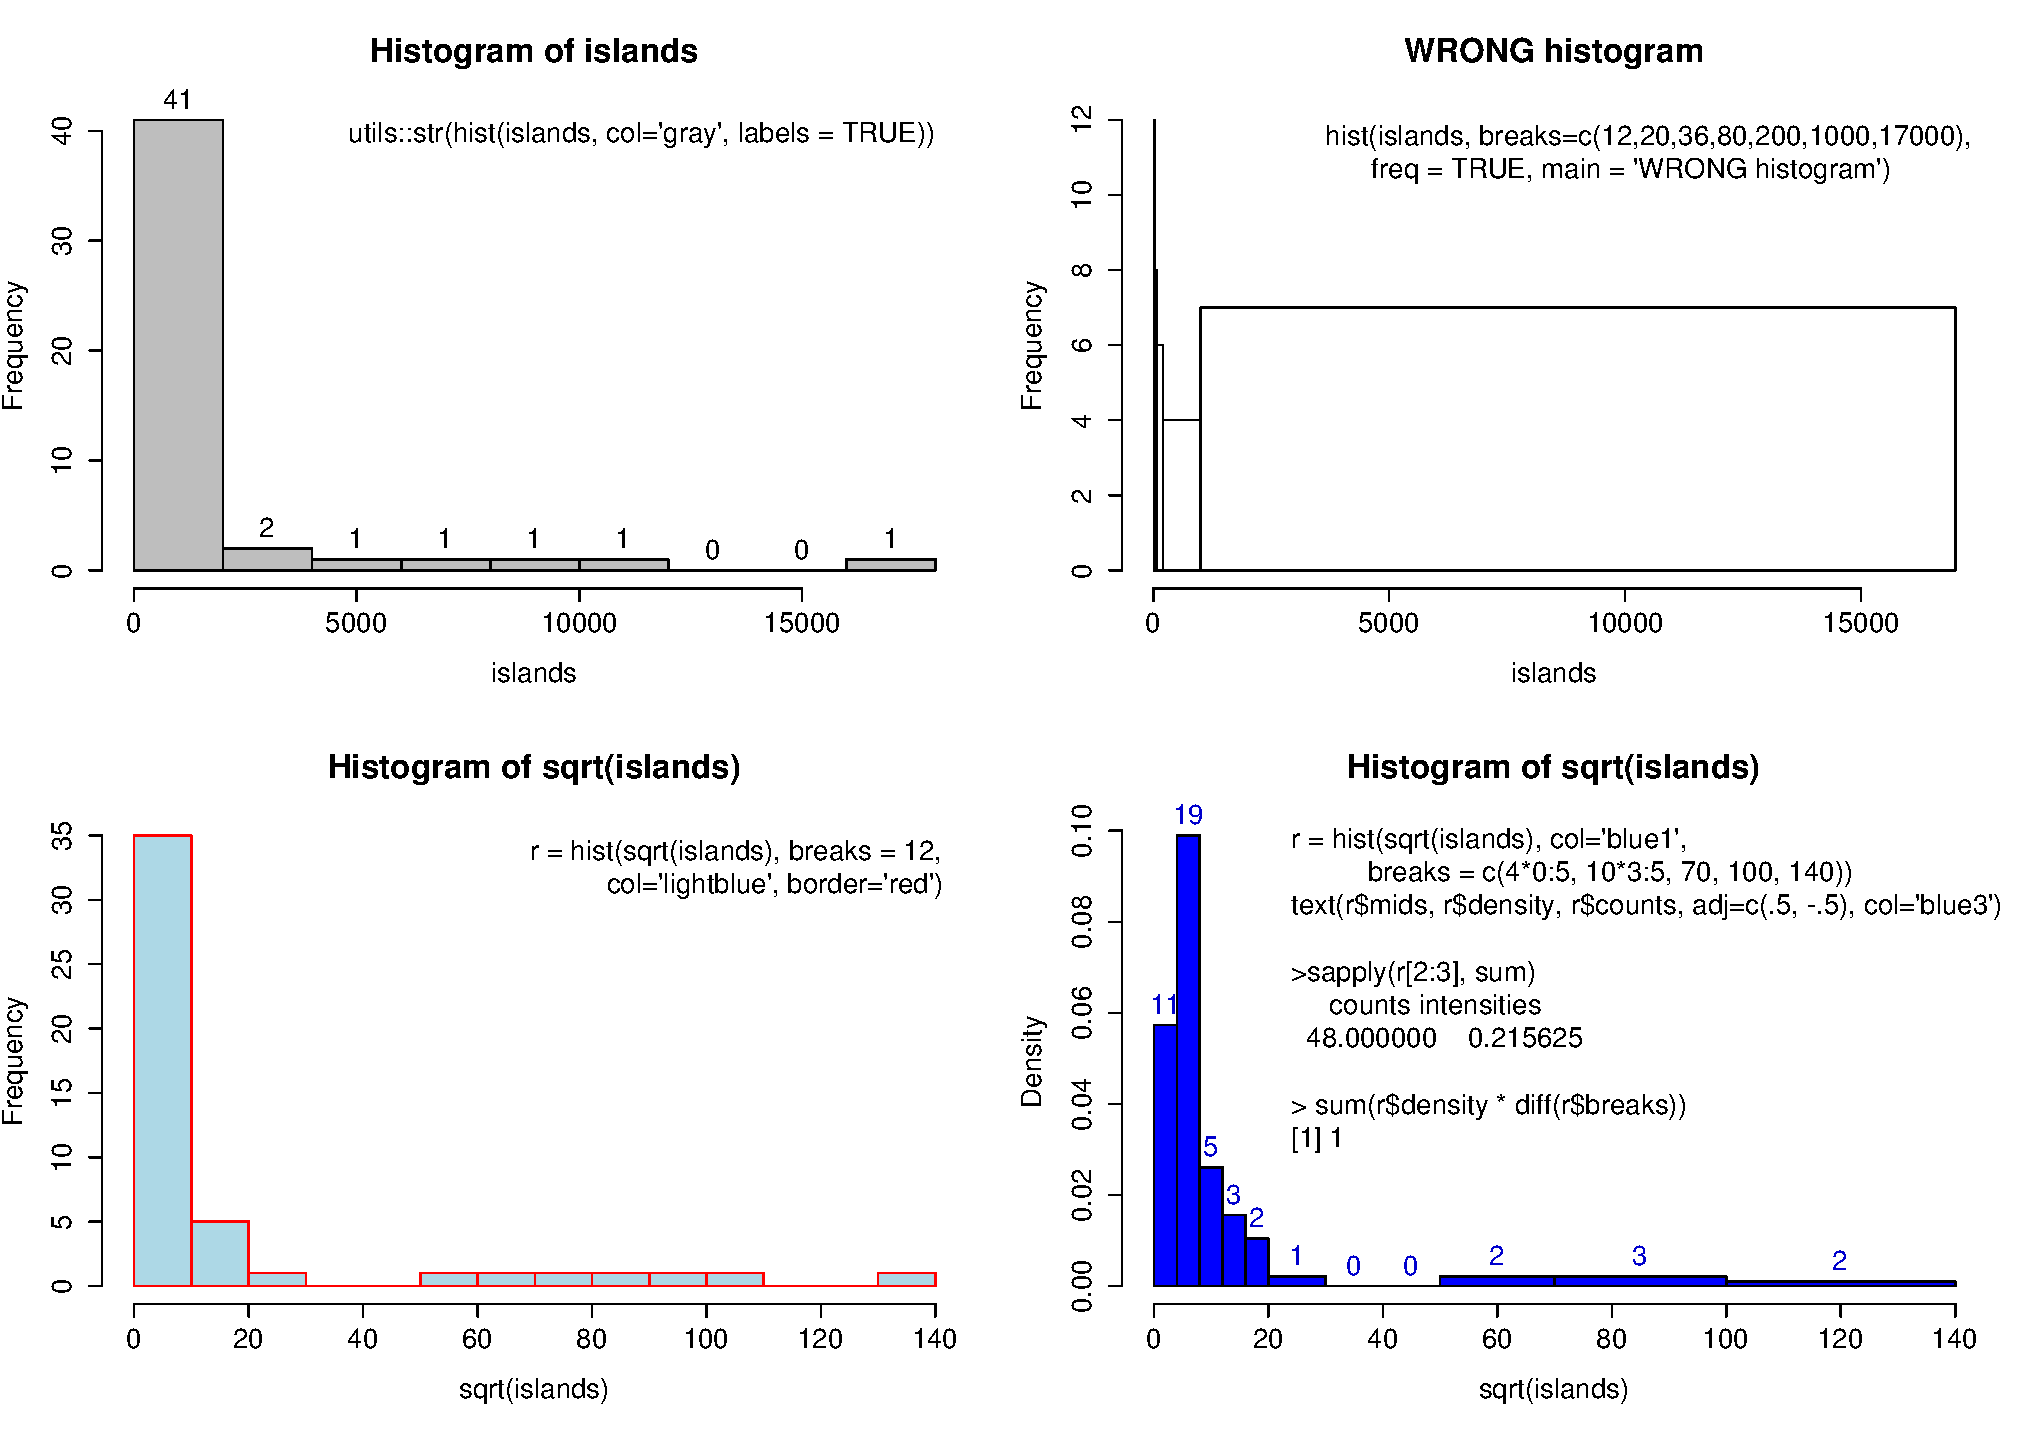
\includegraphics[scale=0.35]{"./01_histograms.pdf}  
\end{frame}


\begin{frame}{Classification of continuous data}
``convert'' continuous data to discrete (choose of bin in histogram),\\
usage: histogram, statistic methods for discrete variables (goodness-of-fit)
\begin{enumerate}
\item same width of bins: 
\item number of bins:  $k = 1+\log_2 n=1+3.3 \log_10 n$
\item width: $h = 2\ (IQR)\ n^{-1/3}$
\item merge bins with less then $5$ values (with neighbor)
\end{enumerate}
\end{frame}



\end{document}


